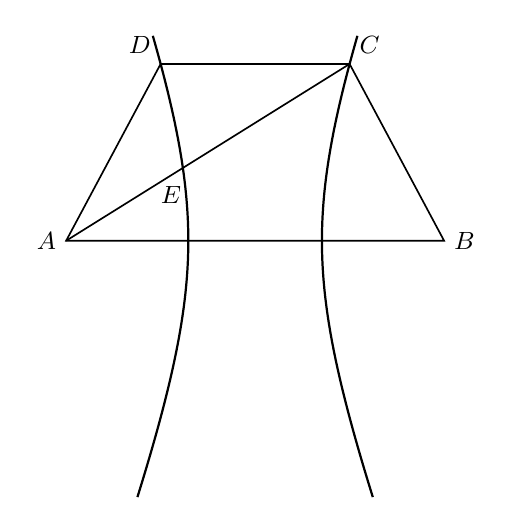
\begin{tikzpicture}[line width=0.6pt, font=\small]
  % foci A,B with c=2.4; hyperbola x^2/a^2-y^2/b^2=1, a=0.8485, b=2.245
  % (lambda=0.7: e^2=8, C=(1.2,2.245) on curve, E=(-0.9176,0.9244) on curve)
  \coordinate (A) at (-2.4,0);
  \coordinate (B) at (2.4,0);
  \coordinate (D) at (-1.2000000000,2.2449944321);
  \coordinate (C) at (1.2000000000,2.2449944321);
  \coordinate (E) at (-0.9176470588,0.9244094720);
  % hyperbola branches from formula x = +/-a*sqrt(1+(y/b)^2)
  
  
  % trapezoid ABCD thin
  \draw (A) -- (B) -- (C) -- (D) -- cycle;
  % diagonal AC thin
  \draw (A) -- (C);
  % labels
  \node[left] at (A) {$A$};
  \node[right] at (B) {$B$};
  \node[above left] at (D) {$D$};
  \node[above right] at (C) {$C$};
  \node[below left,xshift=3pt,yshift=-3pt] at (E) {$E$};
\draw[line width=.8pt] plot[variable=\t,domain=-3.255241926493329:2.6041935411946633,samples=120] ({sqrt(0.72*(1+\t*\t/5.04))},\t);
\draw[line width=.8pt] plot[variable=\t,domain=-3.255241926493329:2.6041935411946633,samples=120] ({-sqrt(0.72*(1+\t*\t/5.04))},\t);
\end{tikzpicture}
